\documentclass{beamer}
%Information to be included in the title page:
% \title{Sample title}
% \author{Anonymous}
% \institute{Overleaf}
\usepackage{xcolor}
\usepackage{booktabs}
\usepackage{graphicx}
\usepackage{subcaption}
\usepackage[]{hyperref}
\usepackage{tikz}
\usepackage{ulem}

\usetheme[]{default}
\begin{document}
\renewcommand{\d}{\: \mathrm{d} }
\newcommand{\e}{\mathrm{e}}


\title[] {Recitation Class 7}

\author[lzx]{Zexi Li}

\institute[email]{lzx12138@sjtu.edu.cn}

\date{2021.07.20}

\frame{\titlepage}

\AtBeginSection[]
{
    \begin{frame}
        \frametitle{Table of Contents}
        \tableofcontents[currentsection]
    \end{frame}
}

\begin{frame}
    \frametitle{Outline}
    \tableofcontents
\end{frame}

\section{Chapter 10 - Fundamentals of the Metal–Oxide–Semiconductor Field-Effect Transistor}
\subsection{The Two-Terminal MOS Structure}
    \begin{frame} \frametitle{Metal–Oxide–Semiconductor}
        \begin{minipage}{\linewidth}
            \begin{minipage}{0.45\linewidth}
                \begin{figure}[H]
                    \centering
                    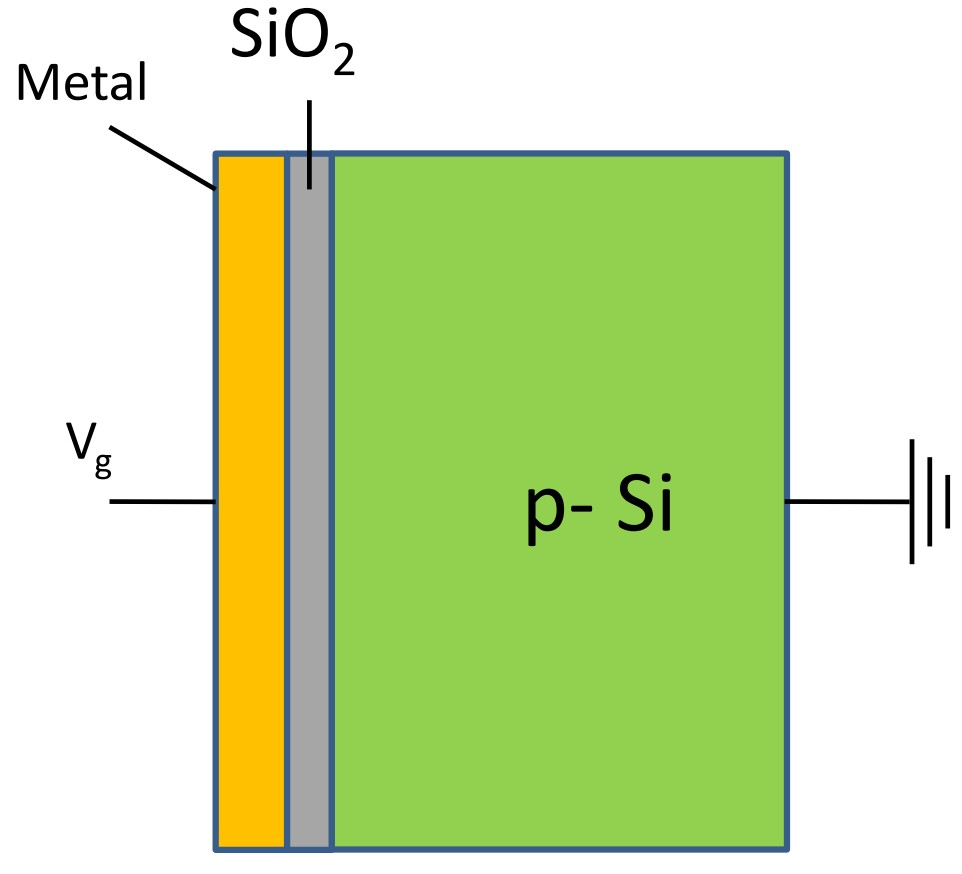
\includegraphics[width=0.8\linewidth]{MOS-graph-horizontal.jpg}
                    \label{fig:MOS-graph-horizontal.jpg}
                \end{figure}
            \end{minipage}
            \begin{minipage}{0.45\linewidth}
                \begin{figure}[H]
                    \centering
                    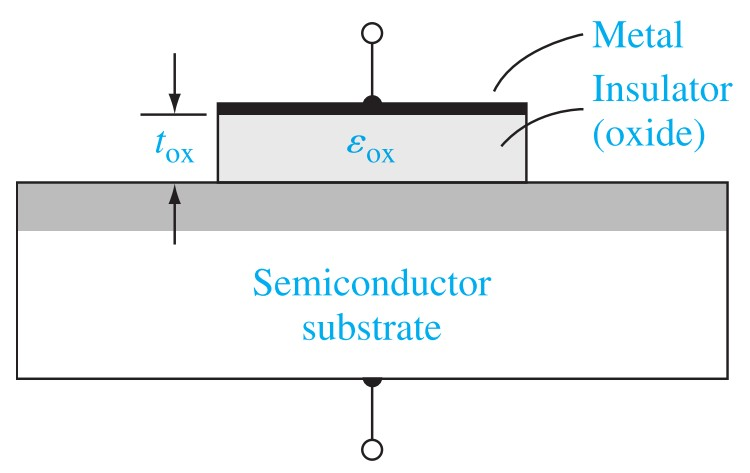
\includegraphics[width=0.8\linewidth]{MOS-graph-vertical.jpg}
                    \label{fig:MOS-graph-vertical.jpg}
                \end{figure}
            \end{minipage}
        \end{minipage}
        \begin{minipage}{\linewidth}
            \begin{figure}[H]
                \centering
                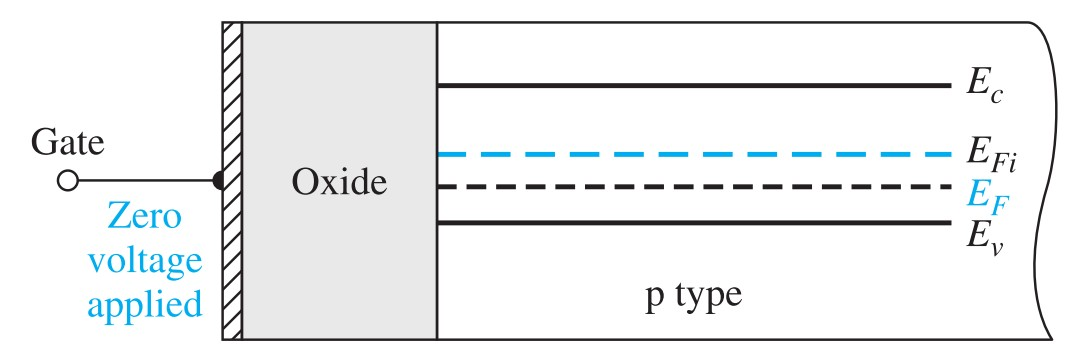
\includegraphics[width=0.6\linewidth]{PMOS-zero-gate-voltage-energy-band-diagram.jpg}
                \label{fig:PMOS-zero-gate-voltage-energy-band-diagram.jpg}
            \end{figure}
        \end{minipage}
    \end{frame}

    \begin{frame} \frametitle{Negative Gate Voltage}
        \begin{figure}[H]
            \centering
            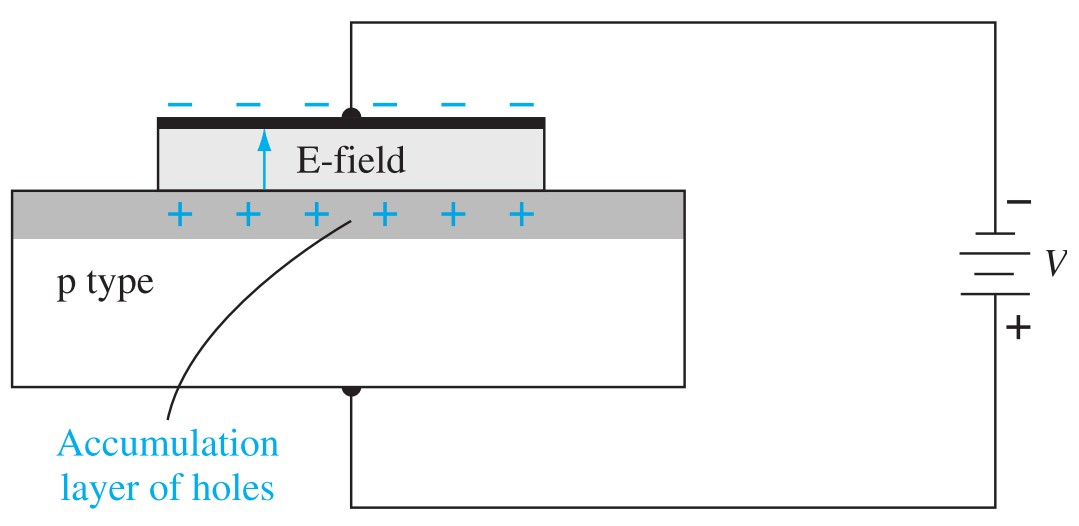
\includegraphics[width=0.6\linewidth]{PMOS-negative-gate-voltage.jpg}
            \label{fig:PMOS-negative-gate-voltage.jpg}
        \end{figure}
    \end{frame}
    \begin{frame} \frametitle{Negative Gate Voltage}
        \begin{figure}[H]
            \centering
            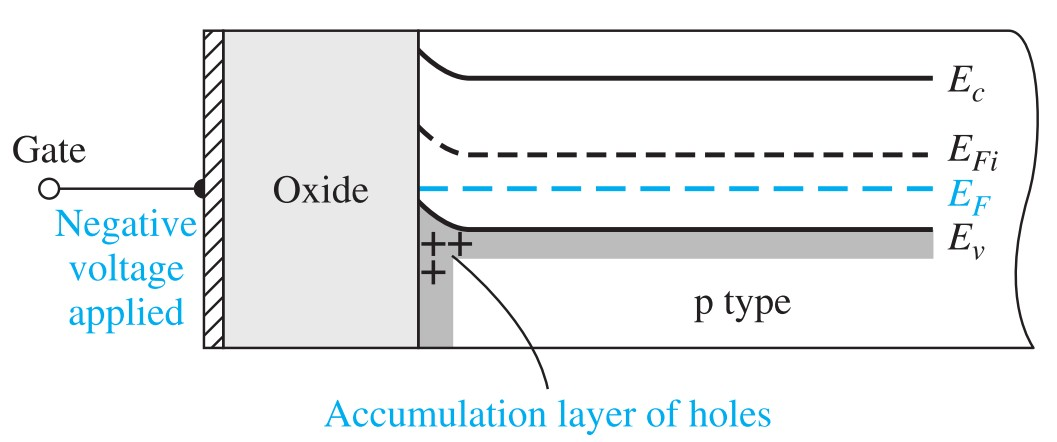
\includegraphics[width=0.6\linewidth]{PMOS-negative-gate-voltage-energy-band-diagram.jpg}
            \label{fig:PMOS-negative-gate-voltage-energy-band-diagram.jpg}
        \end{figure}
    \end{frame}

    \begin{frame} \frametitle{Positive Gate Voltage}
        \begin{figure}[H]
            \centering
            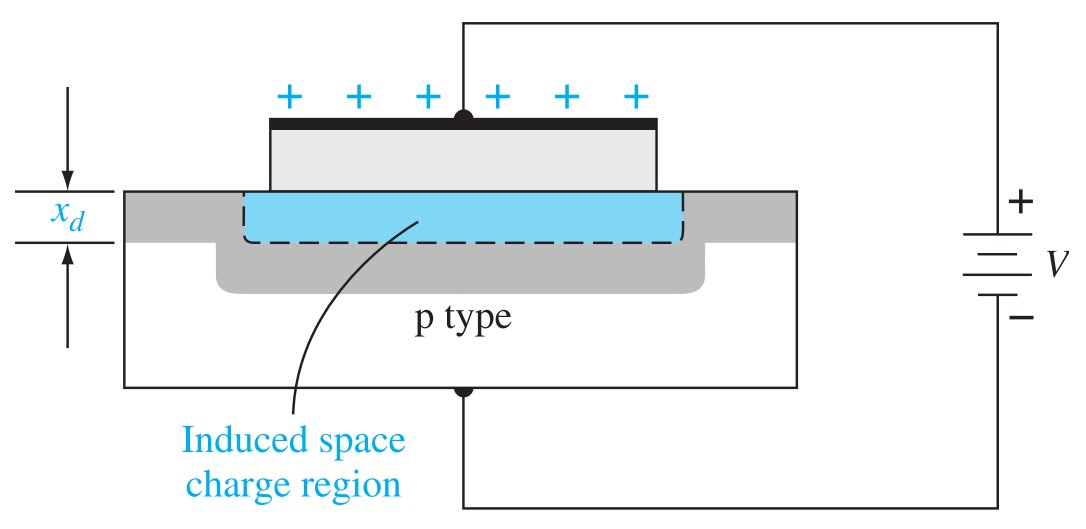
\includegraphics[width=0.6\linewidth]{PMOS-positive-gate-voltage.jpg}
            \label{fig:PMOS-positive-gate-voltage.jpg}
        \end{figure}
    \end{frame}
    \begin{frame} \frametitle{Positive Gate Voltage}
        \begin{figure}[H]
            \centering
            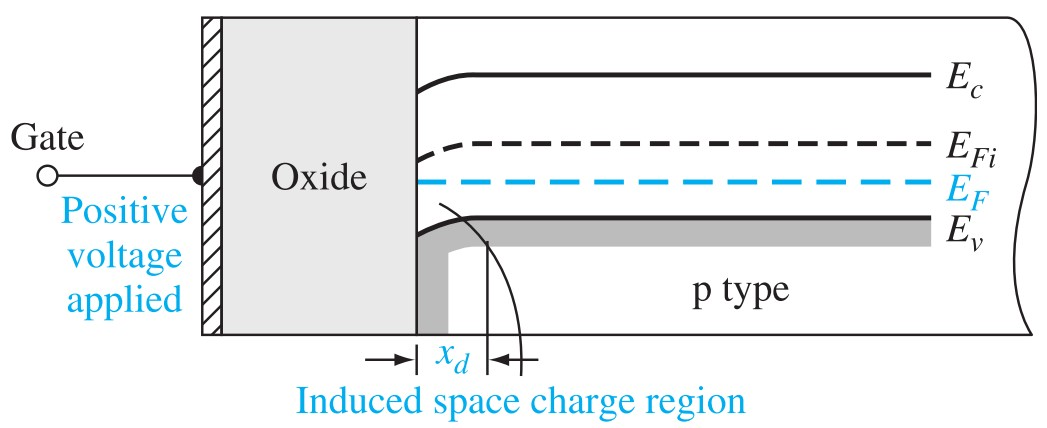
\includegraphics[width=0.6\linewidth]{PMOS-positive-gate-voltage-energy-band-diagram.jpg}
            \label{fig:PMOS-positive-gate-voltage-energy-band-diagram.jpg}
        \end{figure}
    \end{frame}

    \begin{frame} \frametitle{Depletion Layer Thickness}
        \begin{figure}[H]
            \centering
            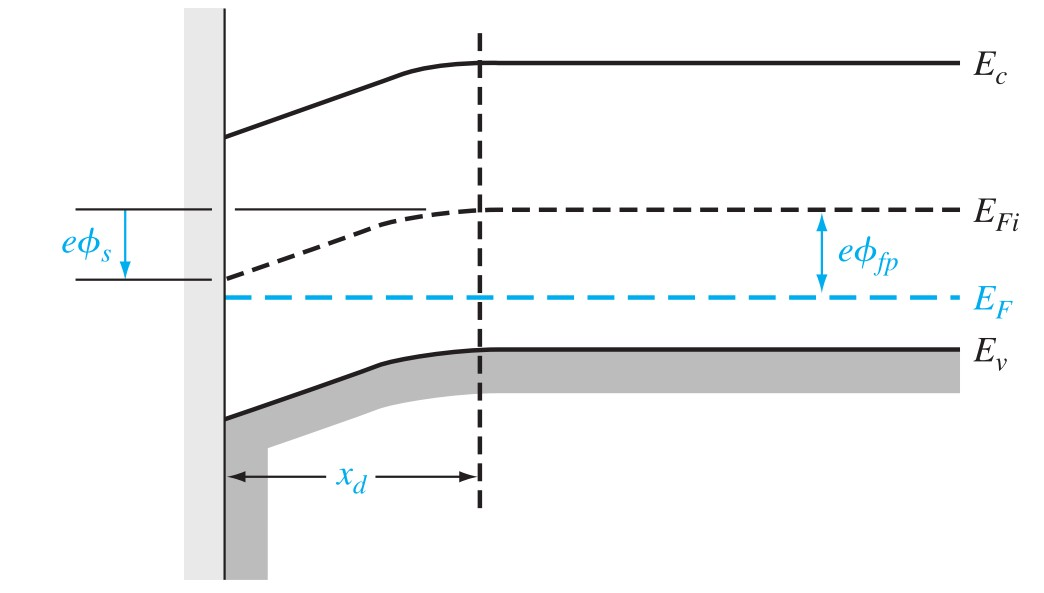
\includegraphics[width=0.6\linewidth]{Energy-band-diagram-PMOS-and-surface-potential.jpg}
            \label{fig:Energy-band-diagram-PMOS-and-surface-potential.jpg}
        \end{figure}
        \begin{equation*}
            \begin{aligned}
                \phi_{fp} &= V_t \ln \left( \frac{N_a}{n_i}  \right) \\
                x_d &= \left( \frac{2 \varepsilon_s \phi_s}{e N_a}  \right)^{1/2} 
            \end{aligned}
        \end{equation*}
        \par $\phi_s$: the surface potential, is the difference (in $V$) between $E_{Fi}$ measured in the bulk semiconductor and $E_{Fi} $ measured at the surface.
    \end{frame}

    \begin{frame} \frametitle{Threshold Inversion Point}
        \begin{figure}[H]
            \centering
            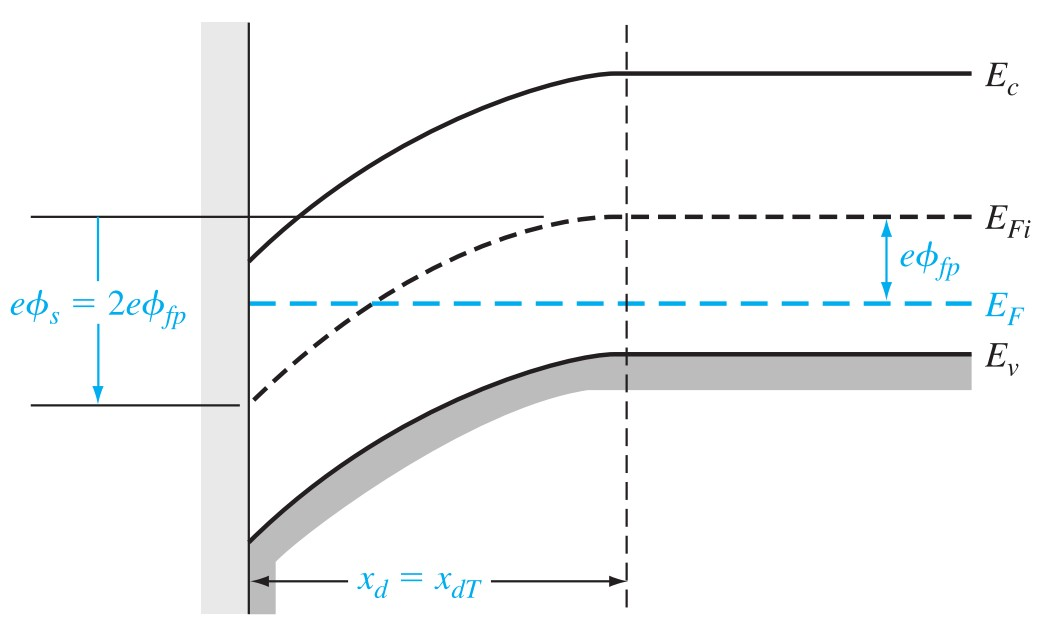
\includegraphics[width=0.6\linewidth]{Threshold-inversion-point.jpg}
            \label{fig:Threshold-inversion-point.jpg}
        \end{figure}
        \begin{equation*}
            \phi_s = 2 \phi_{fp} 
        \end{equation*}
        \begin{equation*}
            \boxed{x_{dT} = \left( \frac{4\varepsilon_s \phi_{fp} }{e N_a} \right)^{1/2}  }
        \end{equation*}
    \end{frame}

\subsection{Capacitance–Voltage Characteristics}
    \begin{frame} \frametitle{Accumulation}
        \begin{figure}[H]
            \centering
            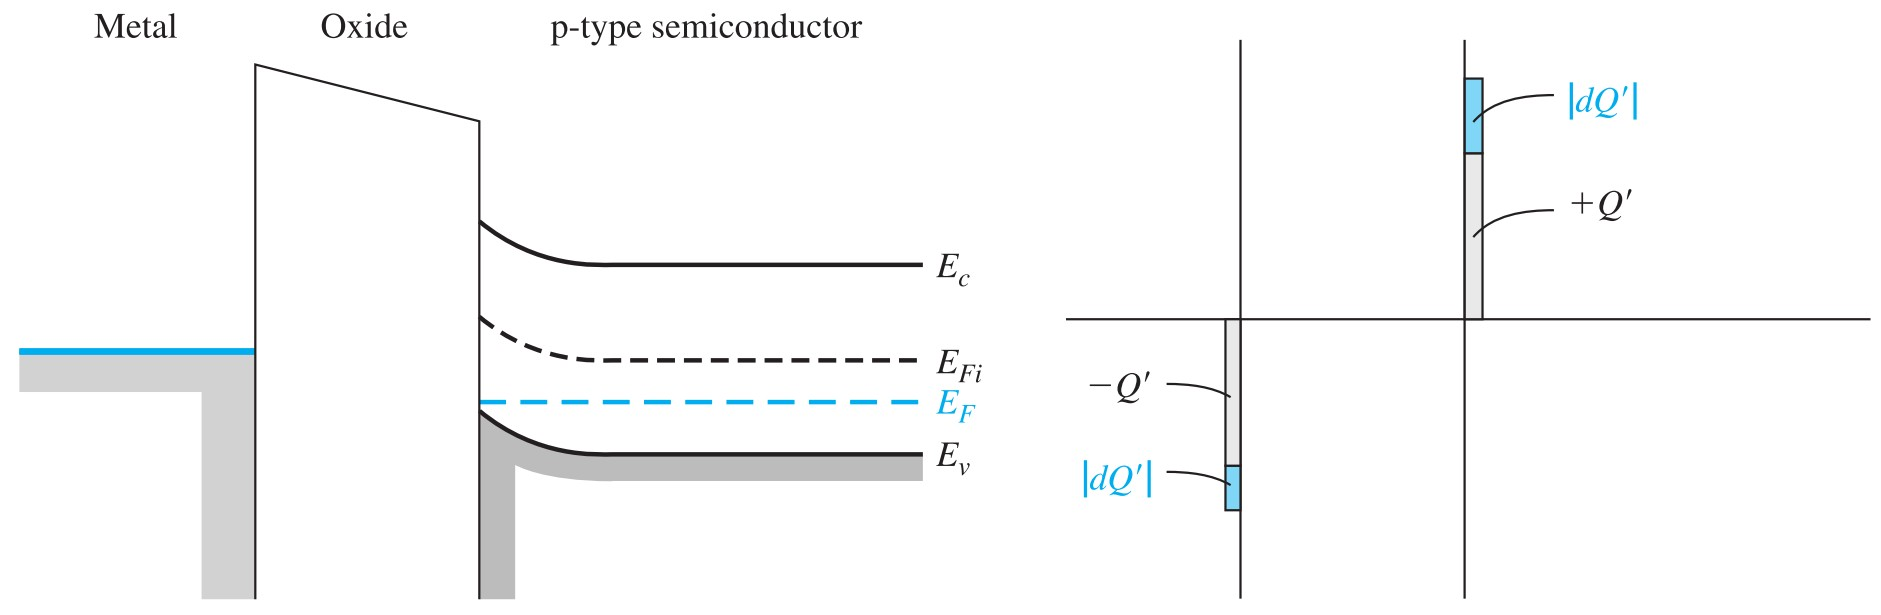
\includegraphics[width=0.9\linewidth]{C-V-accumulation.jpg}
            \label{fig:C-V-accumulation.jpg}
        \end{figure}
        \begin{equation*}
            C^\prime (\text{acc}) = C_{ox} = \frac{\varepsilon_{ox} }{t_{ox} }  
        \end{equation*}
    \end{frame}
    \begin{frame} \frametitle{Depletion}
        \begin{figure}[H]
            \centering
            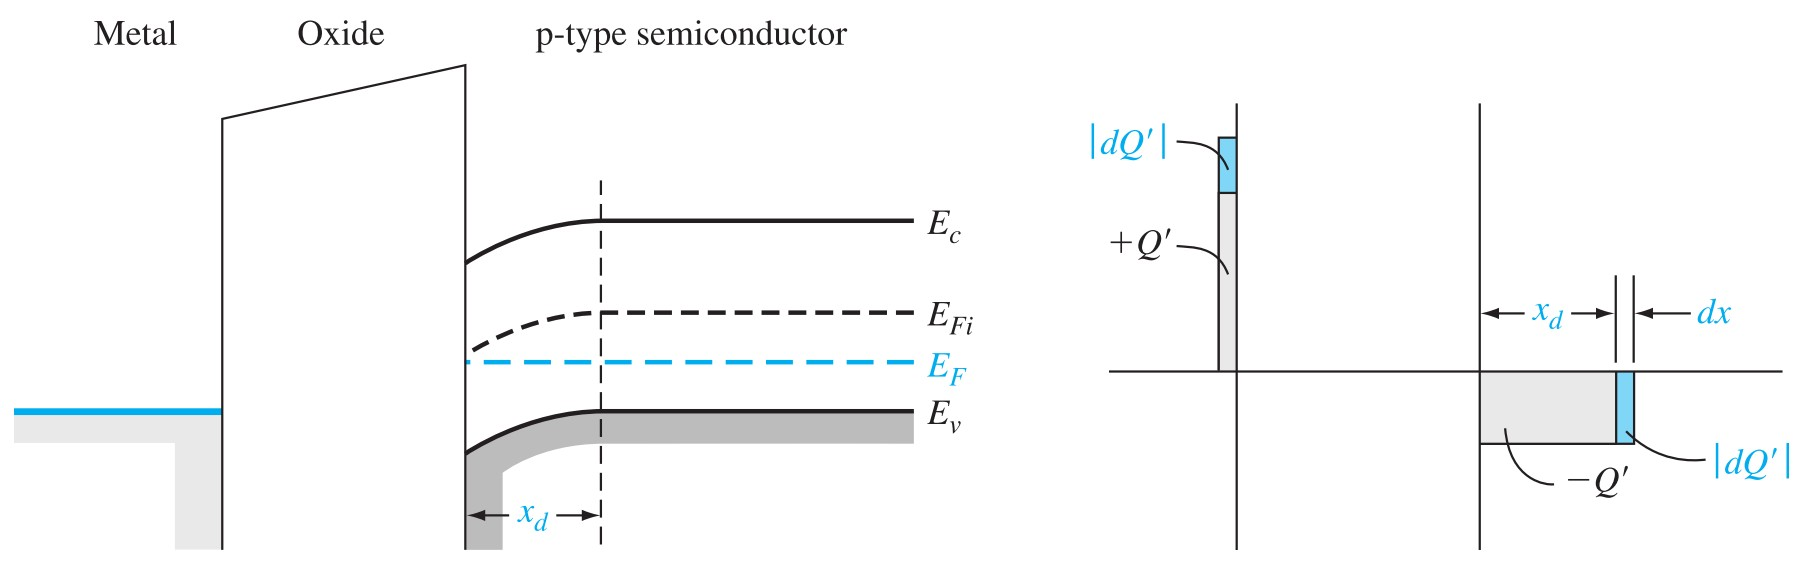
\includegraphics[width=0.9\linewidth]{C-V-depletion.jpg}
            \label{fig:C-V-depletion.jpg}
        \end{figure}
        \begin{equation*}
            \begin{aligned}
                C^\prime (\text{depl}) &= \frac{C_{ox} C^\prime_{SD} }{C_{ox} + C^\prime_{SD} } \\
                &= \frac{\varepsilon_{ox} }{t_{ox} + \left( \frac{\varepsilon_{ox} }{\varepsilon_s}  \right)x_d } 
            \end{aligned}
        \end{equation*}
        \begin{equation*}
            C^\prime_{min} = \frac{\varepsilon_{ox} }{t_{ox} + \left( \frac{\varepsilon_{ox} }{\varepsilon_s}  \right) x_{dT} } 
        \end{equation*}
    \end{frame}
    \begin{frame} \frametitle{Inversion}
        \begin{figure}[H]
            \centering
            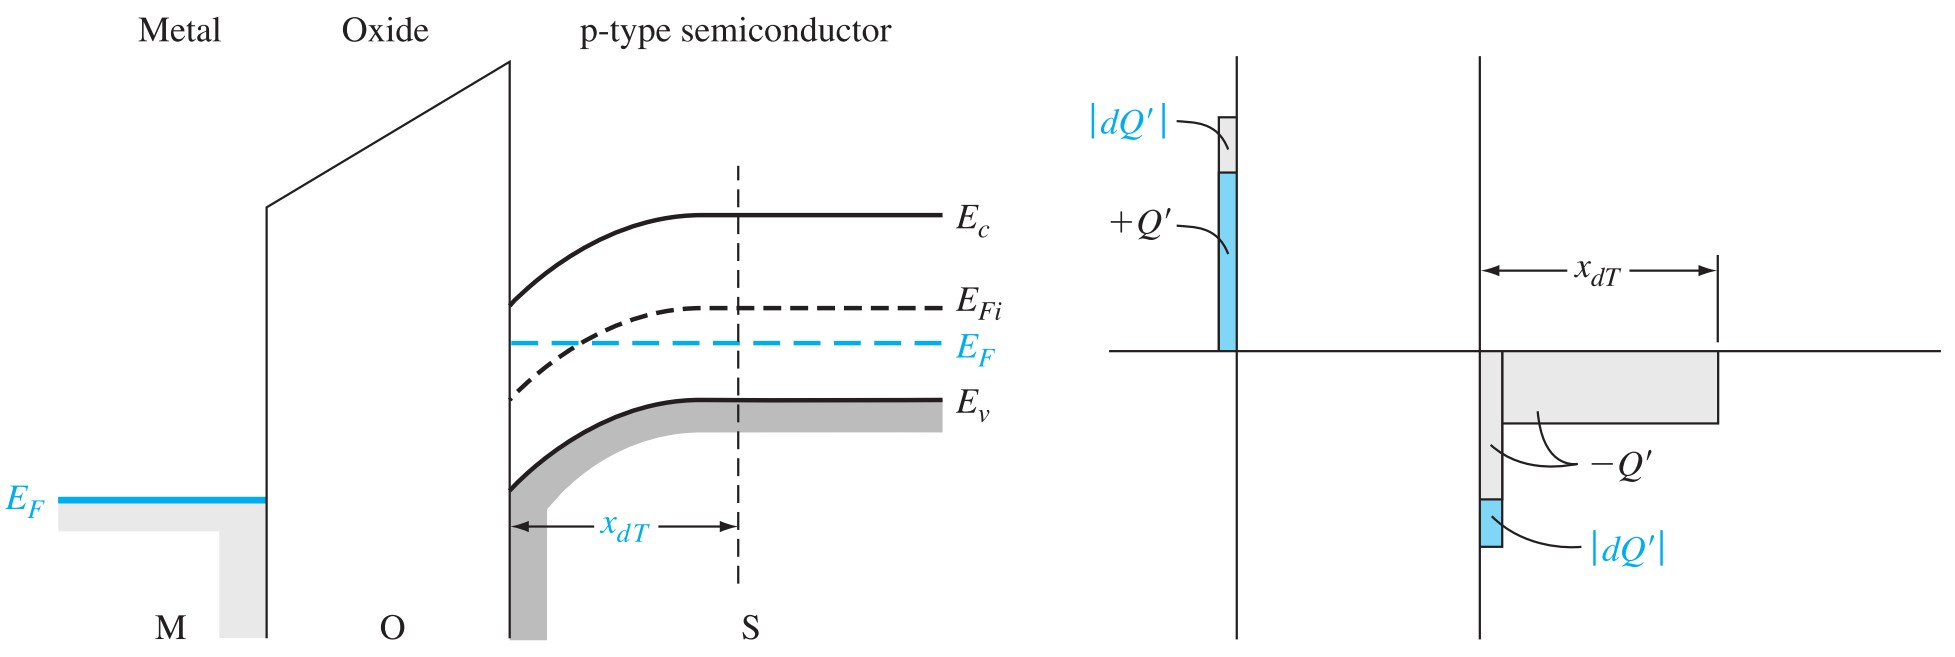
\includegraphics[width=0.9\linewidth]{C-V-inversion.jpg}
            \label{fig:C-V-inversion.jpg}
        \end{figure}
        \begin{equation*}
            C^\prime (\text{inv}) = C_{ox} = \frac{\varepsilon_{ox} }{t_{ox}}
        \end{equation*}
    \end{frame}

    \begin{frame} \frametitle{Ideal Low-Frequency C-V Curve}
        \begin{figure}[H]
            \centering
            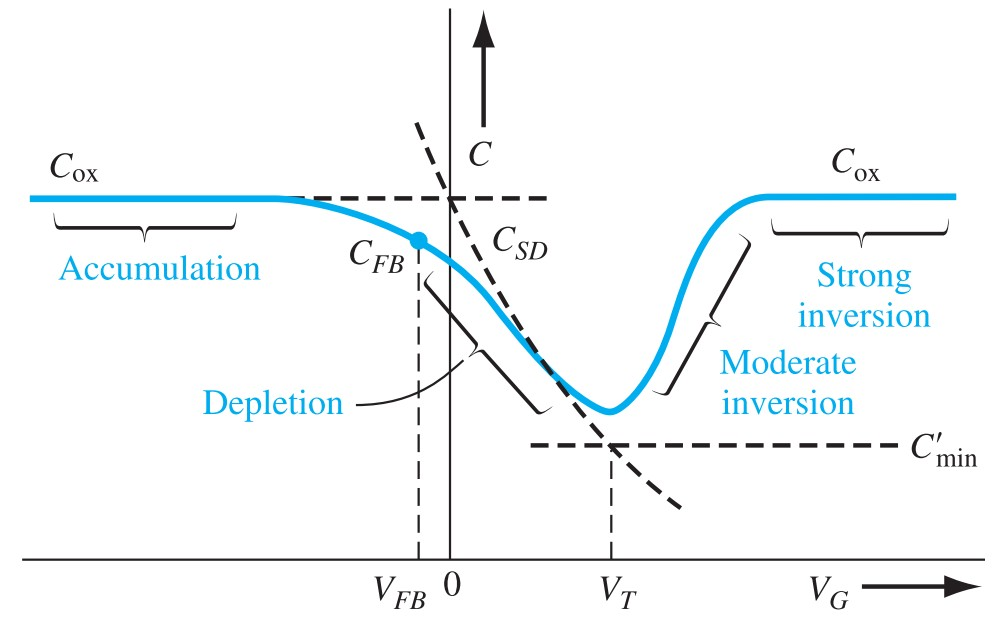
\includegraphics[width=0.8\linewidth]{C-V-graph-low-frequency.jpg}
            \label{fig:C-V-graph-low-frequency.jpg}
        \end{figure}
        \begin{equation*}
            \begin{aligned}
                C^\prime_{FB} = \frac{\varepsilon_{ox} }{t_{ox} + \left( \frac{\varepsilon_{ox} }{\varepsilon_s}  \right) \sqrt{\left( \frac{kT}{e}  \right) \left( \frac{\varepsilon_s}{eN_a}  \right)}} 
            \end{aligned}
        \end{equation*}
    \end{frame}

    \begin{frame} \frametitle{Exercise}
        \par \textcolor{blue}{Objective} Calculate $C_{ox} $, $C^\prime_{min} $ and $C^\prime_{FB} $ for a MOS capacitor.
        \par Consider a p-type silicon substrate at $T = 200K$ doped to $N_a = 10^{16} cm^{-3}$. The oxide is silicon dioxide with a thickness of $t_{ox}  = 18nm = 180 $\r A, and the gate is aluminum. (Example 10.6 on textbook)
        \vspace{1em}
        \par \textbf{\textcolor{blue}{Answer}}: \textcolor{white}{C\_{ox}=1.9175e-7 F/cm\^2, C\_{min}=2.925e-8 F/cm\^2, C\_{FB}=1.091e-7 F/cm\^2}.
    \end{frame}

    \begin{frame} \frametitle{Frequency Effects}
        \par Two sources of electrons
        \begin{enumerate}[1.]
            \item Diffusion of minority carrier electrons.
            \item Thermal generation of electron-hole pairs within the space charge region.
        \end{enumerate}
        \begin{figure}[H]
            \centering
            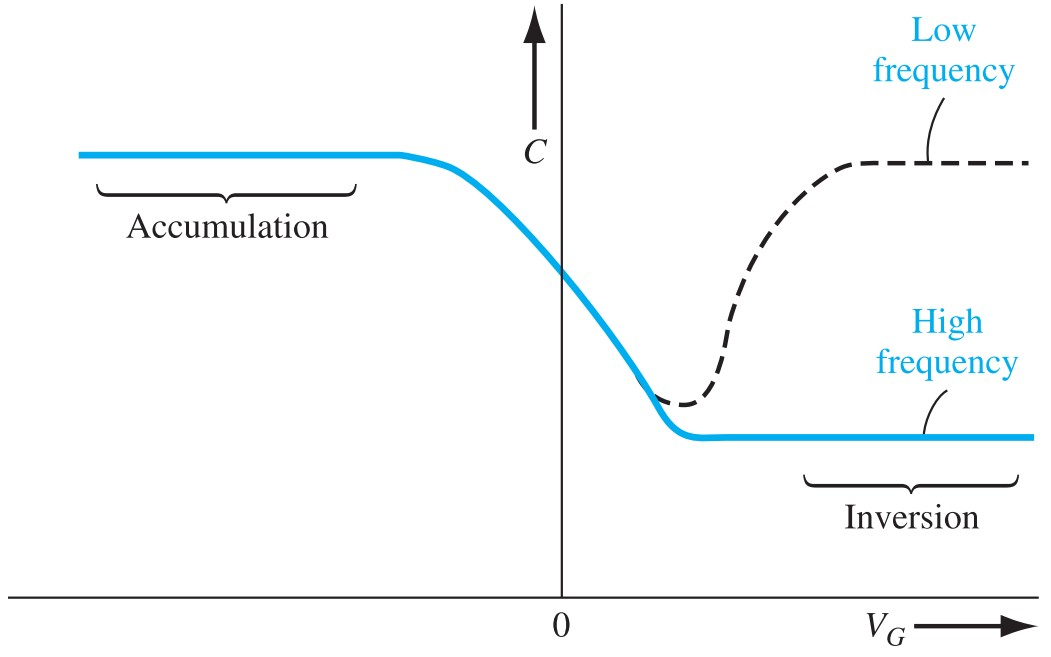
\includegraphics[width=0.8\linewidth]{Frequency-effect.jpg}
            \label{fig:Frequency-effect.jpg}
        \end{figure}
    \end{frame}

\subsection{Non-Ideal Effects}
    \begin{frame} \frametitle{Work Function Difference}
        \begin{figure}[H]
            \centering
            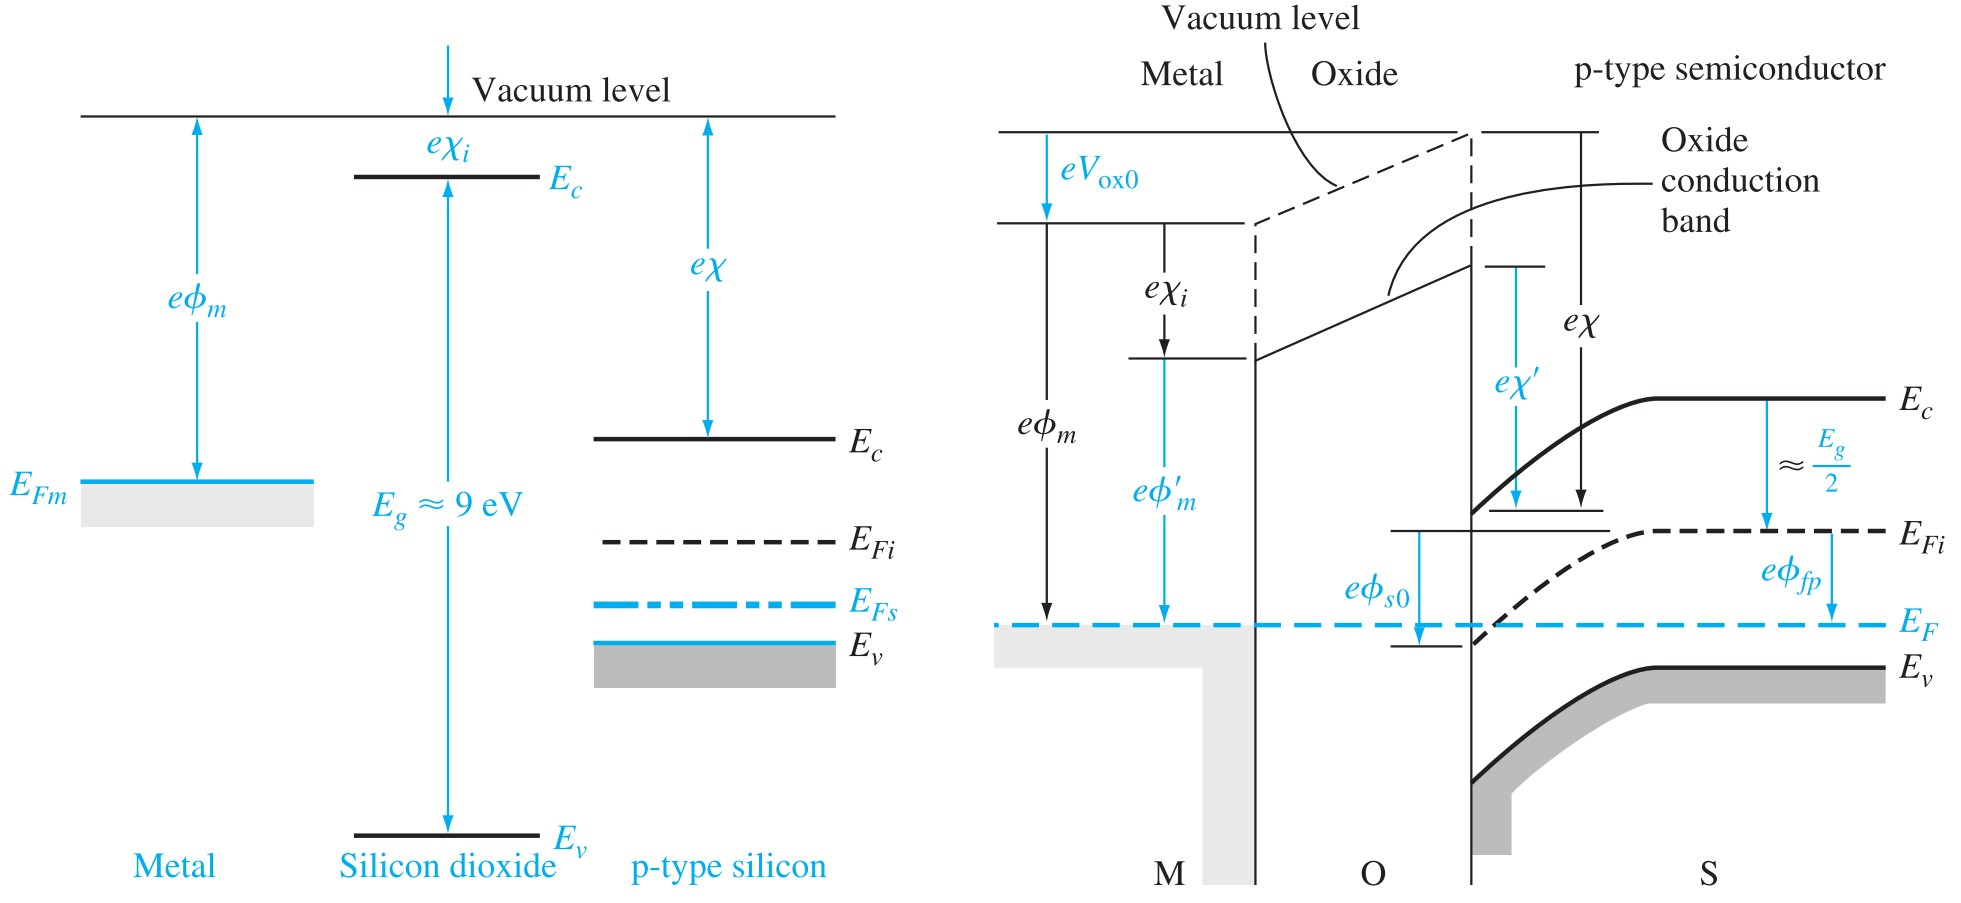
\includegraphics[width=0.9\linewidth]{Work-function-difference.jpg}
            \label{fig:Work-function-difference.jpg}
        \end{figure}
        \begin{equation*}
            \textcolor{gray}{ 
                \begin{aligned}
                    \phi_{ms} &= \phi_m^{\prime} - \left( \chi^\prime + \frac{E_g}{2e} + \phi_{fp}  \right) \\
                    \phi_{ms} &= \phi^\prime_m - \left( \chi^\prime + \frac{E_g}{2e} - \phi_{fn}  \right)
                \end{aligned}
            }
        \end{equation*}
        \textcolor{gray}{Not required}. 
    \end{frame}

    \begin{frame} \frametitle{Fixed Charge}
        \begin{minipage}{\linewidth}
            \begin{minipage}{0.45\linewidth}
                \begin{figure}[H]
                    \centering
                    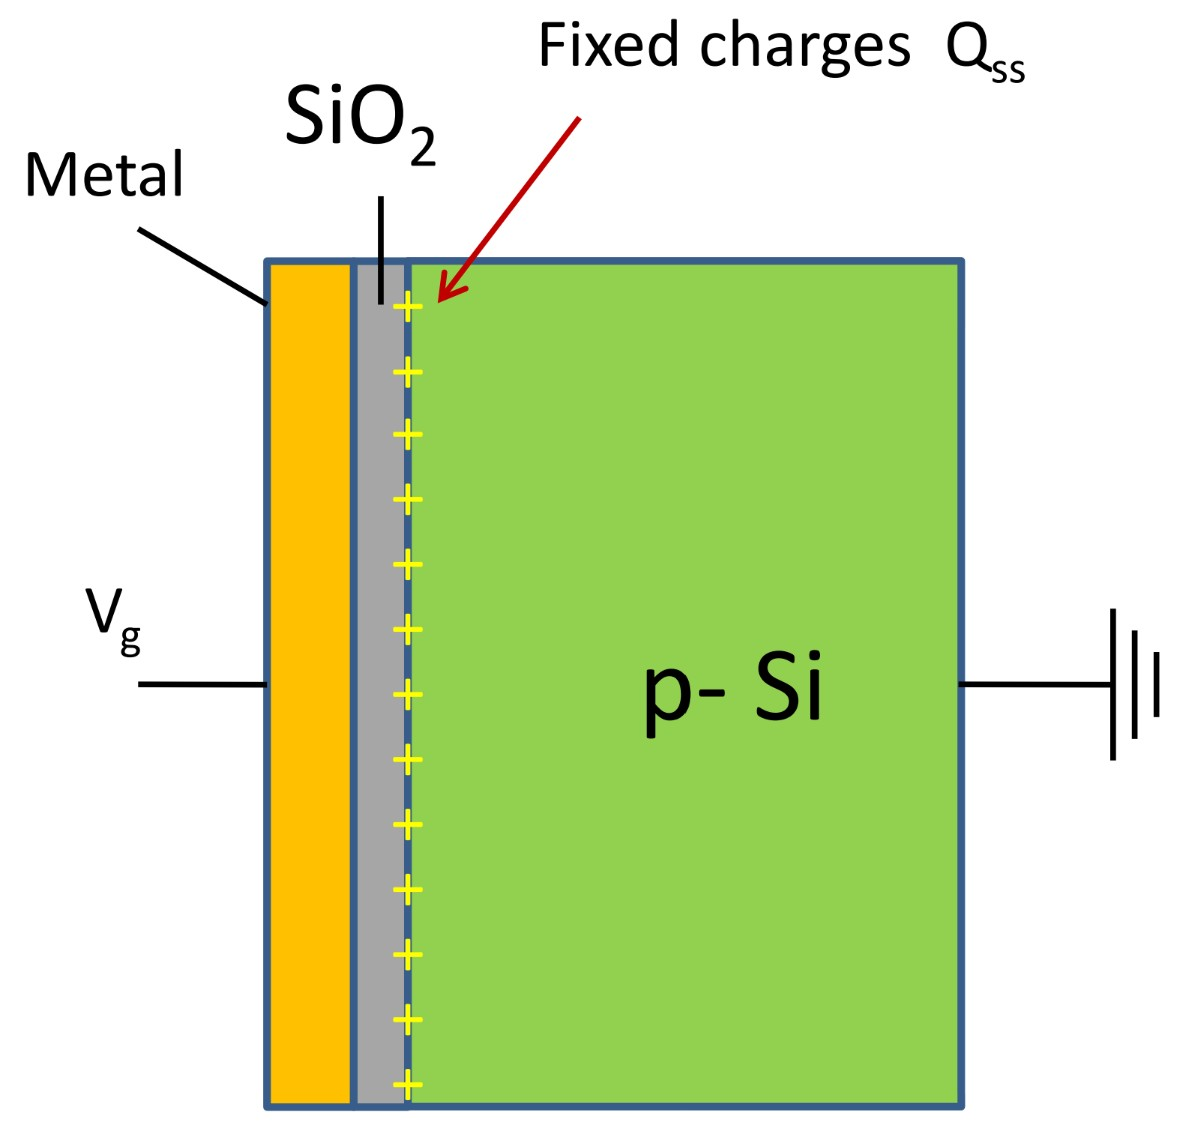
\includegraphics[width=0.9\linewidth]{Fixed-charge.jpg}
                    \label{fig:Fixed-charge.jpg}
                \end{figure}
            \end{minipage}
            \begin{minipage}{0.45\linewidth}
                \begin{figure}[H]
                    \centering
                    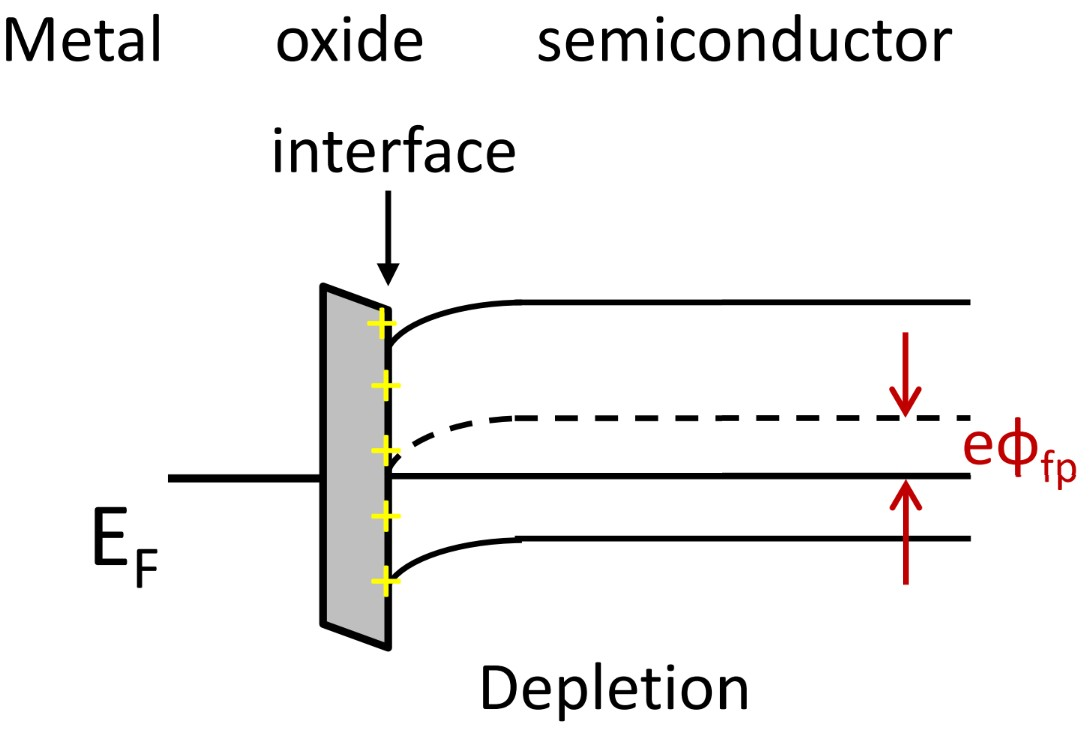
\includegraphics[width=0.9\linewidth]{Fixed-charge-energy-band-diagram.jpg}
                    \label{fig:Fixed-charge-energy-band-diagram.jpg}
                \end{figure}
            \end{minipage}
        \end{minipage}
    \end{frame}
    \begin{frame} \frametitle{Adjustment on $V_T$}
        \begin{equation*}
            \boxed{
            \begin{aligned}
                \left| Q^\prime_{SD} (\text{max}) \right| &= eN_a x_{dT} = 2 \sqrt{e \varepsilon_s N_a \phi_{fp} } \\
                V_{TN} &= \frac{\left| Q^\prime_{SD} (\text{max}) \right|}{C_{ox} } + V_{FB} + 2 \phi_{fp}  \\
                V_{TP} &= - \frac{\left| Q^\prime_{SD} (\text{max}) \right|}{C_{ox} } + V_{FB} - 2 \phi_{fn}  \\
                V_{FB} &= \phi_{ms} - \frac{Q^\prime_{ss} }{C_{ox}}\cdot \frac{x}{d} 
            \end{aligned}
            }
        \end{equation*}
    \end{frame}

    \begin{frame} \frametitle{Surface States}
        \begin{minipage}{\linewidth}
            \begin{minipage}{0.45\linewidth}
                \begin{figure}[H]
                    \centering
                    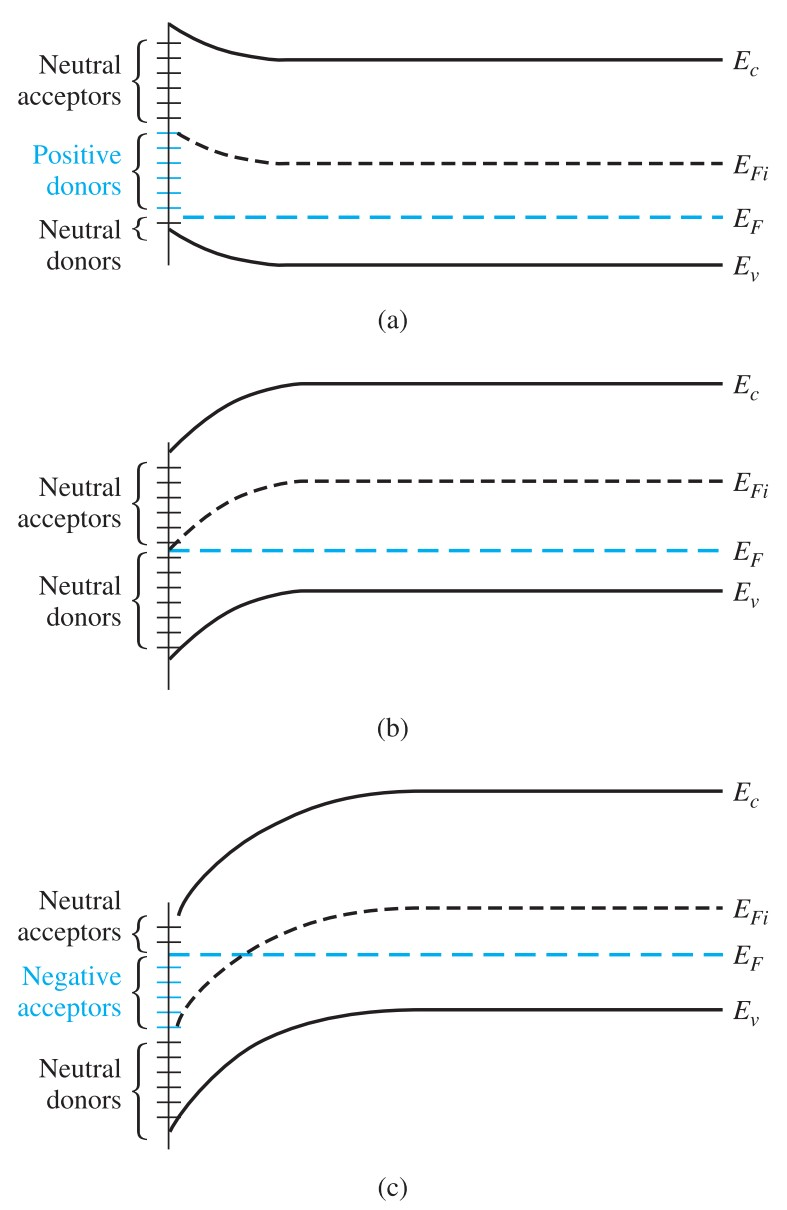
\includegraphics[width=\linewidth]{Surface-states-midgap.jpg}
                    \label{fig:Surface-states-midgap.jpg}
                \end{figure}
            \end{minipage}
            \begin{minipage}{0.45\linewidth}
                \begin{figure}[H]
                    \centering
                    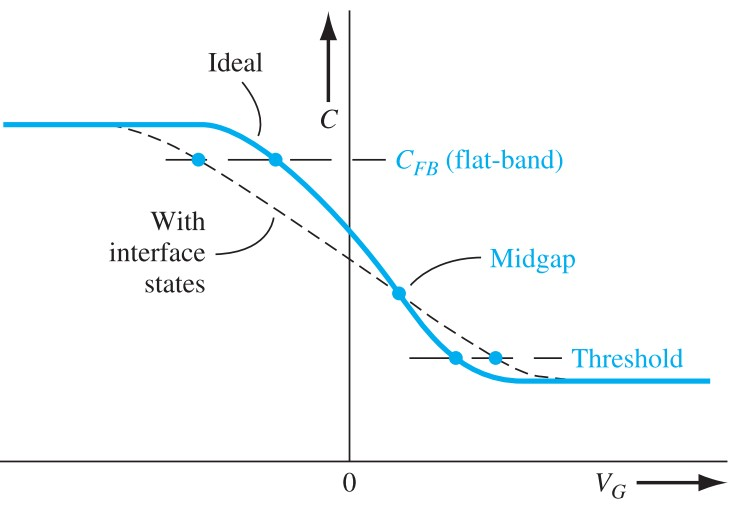
\includegraphics[width=0.9\linewidth]{Surface-states.jpg}
                    \label{fig:Surface-states.jpg}
                \end{figure}
            \end{minipage}
        \end{minipage}
    \end{frame}

    \begin{frame} \frametitle{Example}
        \par \textcolor{blue}{Objective} Calculate the threshold voltage of a MOS system using an aluminum gate. 
        \par Consider a p-type silicon substrate at $T = 300K$ doped to $N_a = 10^{15} cm^{-3} $. Let $Q^\prime_{ss} = 10^{10} cm^{-2} $, $t_{ox} = 12cm = 120$\r{A}, and assume the oxide is silicon dioxide. $\phi_{ms} = -0.88 V$. (Example 10.4 on textbook)

        \vspace{1em}
        \par \textbf{\textcolor{blue}{Answer}}: \textcolor{white}{V\_{TN} = -0.262 V}.
    \end{frame}

    \begin{frame} 
        \begin{center}
            \Large\textcolor{blue}{End}
        \end{center}
    \end{frame}
\end{document} 